% created by Uwe Schadewald
% modified by Mathias Kuntze and Ahmet Uysal
% Add, handout to documentclass arguments for condensed pdf
\documentclass[presentation, 8pt, mathserif, t]{beamer} % , aspectratio=169
\usepackage[english]{babel}
\usepackage{pgf,graphicx}
\usepackage{amsmath, amssymb}
\usepackage[utf8]{inputenc}
\usepackage{lmodern}
\usepackage{palatino}
\usepackage{multimedia}
\usepackage{pgfpages} 
\usepackage{tikz}
\usepackage{datetime}
\pdfoptionpdfminorversion=5

\usepackage{caption}
\usepackage{subcaption}
% if else
\usepackage{ifthen}
% extend table options
\usepackage{tabularx} 
\usepackage{booktabs}
\usepackage{multicol}
\usepackage{multirow}
\usepackage{eso-pic}  % package to set background image
\usepackage[calc]{picture}

% Packages and stuff for ToDo list like itempoints
\usepackage{pifont}
\newcommand{\cmark}{\ding{51}}%
\newcommand{\xmark}{\ding{55}}%
\newcommand{\open}{$\square$}
\newcommand{\done}{\rlap{$\square$}{\raisebox{1pt}{\large\hspace{1.5pt}\cmark}}\hspace{-2.5pt}}
\newcommand{\wontfix}{\rlap{$\square$}{\raisebox{1pt}{\large\hspace{1.5pt}\xmark}}}
\newcommand{\notsure}{\rlap{$\square$}{\raisebox{0.8pt}{\large\hspace{1.5pt}\textbf{?}}}}



% side bar and footer
\setbeamertemplate{headline}{	
	\leavevmode
	\vspace{-4em}	
	\hbox{		
		\begin{beamercolorbox}[wd=0.85\paperwidth,ht=10ex,dp=8ex,center]{}%			
			% navigation with subsections as dots
			\hspace{3.5em}\insertnavigation{0.7\paperwidth}{\hskip0pt plus1fill} % add navigation in footer						
			% navigation with sections, no subsections
			% \insertsectionnavigationhorizontal{0.6\paperwidth}{\hskip0pt plus1fill}{} \\ % add navigation in footer}
			
		\end{beamercolorbox} 				
	}
	\vskip0pt
}


\setbeamertemplate{footline}{	
	\leavevmode
	\vspace{-3em}
	\hbox{
		\begin{beamercolorbox}[wd=.33\paperwidth,ht=2.25ex,dp=1ex,left]{author in head/foot}%
			\hspace{5em}
			\insertshortauthor
		\end{beamercolorbox}
		\begin{beamercolorbox}[wd=.33\paperwidth,ht=2.25ex,dp=1ex,center]{title in head/foot}%
			\insertshorttitle \ - \insertshortsubtitle
		\end{beamercolorbox}	
		\begin{beamercolorbox}[wd=0.30\paperwidth,ht=10ex,dp=8ex,right]{pagenumber in head/foot}			 	
			\insertframenumber % add page numbers
		\end{beamercolorbox}
	}			
	\vskip0pt
}



\setbeamertemplate{frametitle}{
	\ifthenelse{\equal{\insertframesubtitle}{}}{
		\vspace{0.6cm}
		\huge{\insertframetitle}
	}{
		\vspace{0.6cm}
		\small{\insertframetitle}\\
		\vspace{0.3cm}
		\huge{\insertframesubtitle}
    }		
}

	
% enumerate sections
\setbeamertemplate{section in head/foot}{\hfill\insertsectionheadnumber.~\insertsectionhead}
%\setbeamertemplate{section in head/foot shaded}{\color{structure!50}\hfill\insertsectionheadnumber.~\insertsectionhead}
\setbeamertemplate{section in toc}{\inserttocsectionnumber.~\inserttocsection}

%enumerate subsections
\setbeamertemplate{subsection in head/foot}{\hfill\insertsubsectionheadnumber.~\insertsubsectionhead}
\setbeamertemplate{subsection in head/foot shaded}{\color{structure!50}\hfill\insertsubsectionheadnumber.~\insertsubsectionhead}
%\setbeamertemplate{subsection in toc}[subsections numbered]
\setbeamertemplate{subsection in toc}{\vskip0.5em\leftskip=2em\inserttocsubsection\par}

%--------------------------Common------------------------------------------------------
\setbeamercovered{transparent} % make the beamer theme invisible
\usefonttheme{structurebold}
\beamertemplatenavigationsymbolsempty % set navigations helper function to off
\setbeamertemplate{bibliography item}[text]
\setbeamertemplate{note page}[plain]

%\setlist[itemize,1]{label={$\bullet$}} % \item are using bullets
\setbeamertemplate{itemize items}[circle]
	
	

	
% create a new command to show it on two screens
% I'm using dspdfviewer.
\newcommand{\setDualView} {
	\setbeameroption{show notes on second screen=right}
}

%\AtBeginSection[]{\subsection{}}
\newcommand{\addcite}[1]{%
	\AddToShipoutPictureFG*{%
		\AtPageLowerLeft{%
			\put(0.90\paperwidth,5em){											
				\tiny{
					\cite{#1} 
				}			
			}
		}
	}	
}

% insert a frame with references -> use bibtex
\newcommand{\insertReferenceFrame}[3]{%
	\section{#1}
	\begin{frame}[allowframebreaks]
		\frametitle{#1}
		\bibliographystyle{#2}
		\bibliography{#3}
	\end{frame}	
}

\AtBeginSection[]{\subsection{}}
	





\usepackage{../KU-Beamer-Template/style/koc} 
\usepackage{minted}
\usepackage{upquote}
\usepackage{graphicx}

\title{KOLT Python}
% https://www.geeksforgeeks.org/difference-method-function-python/
\subtitle{Functions} 
\newdate{date}{11}{03}{2019}
\date{\displaydate{date}}
\author{İpek Köprülülü}

\titlegraphic{
\includegraphics[scale=0.2]{../KU-Beamer-Template/style/images/logo_kolt.eps}}

\setbeamercovered{invisible} % transparent
\makeatletter
\let\@@magyar@captionfix\relax
\makeatother
\begin{document}
    \maketitle

    \frame{\frametitle{Agenda}\tableofcontents}

    \section{Recap}
        \begin{frame}{Lists}
            \begin{itemize}
                \LARGE
                \item Group values together. \texttt{my\_values = [1, \textquotesingle a\textquotesingle, None]}
                \item You can think of each element as a variable, accessed by \textbf{indexing}
                \item You can do everything you do to variables to list elements:
                    \begin{itemize}
                        \Large
                        \item Assign new values: \texttt{my\_values[0] = 3}
                        \item Use shorthand assignment operators: \texttt{my\_values[1] += \textquotesingle bc\textquotesingle}
                        \item Learn their type: \texttt{type(my\_values[2]) \# => <class \textquotesingle NoneType\textquotesingle>}
                        \item Change their type: \texttt{my\_values[2] = True}
                        \item Compare their value: \texttt{if my\_values[0] == my\_values[1]: ...}
                    \end{itemize}
                \item What happens when we call \texttt{my\_values[3] = 3}? \texttt{\# => \textbf{IndexError}}
            \end{itemize}
        \end{frame}

        \begin{frame}{List Indexing}
            \LARGE
            Access elements at a particular index
            \begin{columns}
            \begin{column}{0.5\textwidth}
                \vspace{-5mm}
                \begin{figure}[H]
                    \bigskip
                    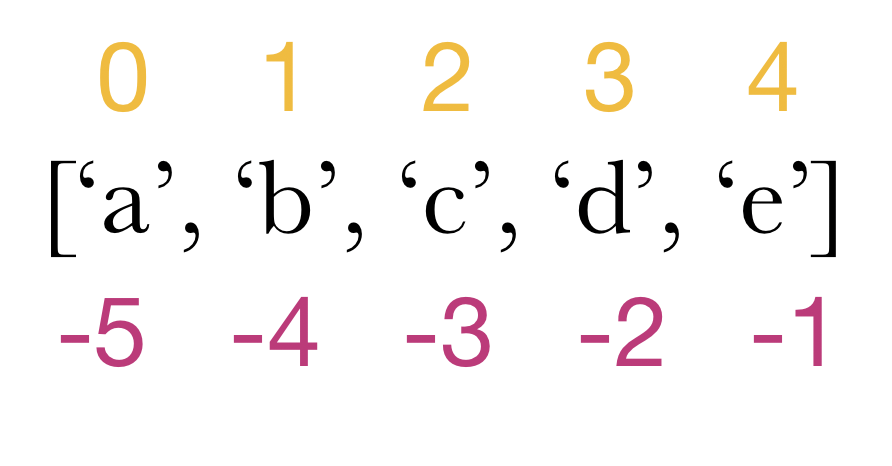
\includegraphics[width=70mm]{../Lecture3/code-examples/index.png}
                    \end{figure}    
            \end{column}
            \begin{column}{0.5\textwidth}
                \inputminted[frame=single,framesep=2pt, lastline=8]{python3}{../Lecture3/code-examples/index.py}
            \end{column} 
            \end{columns}
        \end{frame}

        \begin{frame}{List Slicing}
            \LARGE
            Access collection of elements by specifying \textbf{\texttt{[start:stop:step]}}\\
            Gives a list, even when number of elements is not bigger than 1.
            \normalsize
            \vspace{-2mm}
            \begin{columns}
                \begin{column}{0.5\textwidth}
                    \inputminted[frame=single,framesep=2pt,lastline=9]{python3}{../Review1/code-examples/slicing.py}                        
                \end{column}                
                \begin{column}{0.5\textwidth}
                    \inputminted[frame=single,framesep=2pt,firstline=10]{python3}{../Review1/code-examples/slicing.py}                                
                \end{column}
            \end{columns}
            \vspace{2mm}
            \LARGE
            Slices with \texttt{step} = 1 are called \textbf{Basic Slice}.\\
            Slices with \texttt{step != 1} are called \textbf{Extended Slice}.
        \end{frame}

        \begin{frame}{List Mutation}
            \LARGE
            \textbf{\texttt{list.append(x)}}: Append x to end of the sequence\\
            \textbf{\texttt{list.insert(i, x)}}: Insert x to index i\\
            \textbf{\texttt{list.pop(i=-1)}}: Remove and return element at index i\\
            \textbf{\texttt{list.remove(x)}}: Remove first occurrence of x\\
            \textbf{\texttt{list.extend(iterable)}}: Add all elements in iterable to end of list\\
            \textbf{\texttt{list[i] = new\_value}}: Update value of index i with new value\\
            \textbf{\texttt{list[basic\_slice] = iterable}}: Change elements in basic slice with elements in iterable, sizes can be different: \texttt{numbers[:] = []}\\
            \textbf{\texttt{list[extended\_slice] = iterable}}: Change elements in extended slice with elements in iterable 1-1, sizes must be equal.\\
        \end{frame}

        \begin{frame}{Some Other List Operations}
            \LARGE
            \textbf{\texttt{in}} operator: Check whether an element is in list. \texttt{3 in numbers} $\Rightarrow$ \texttt{True}\\
            \textbf{\texttt{len(list)}}: Returns the length of list(and other collections).\\
            \textbf{\texttt{list.index(value, start=0, stop=len(list))}}: Return first index of value.\\
            \textbf{\texttt{list.count(value)}}: Count number of occurrences of value in list.\\
            \textbf{\texttt{list.reverse()}}: Reverse the list (in-place)\\
            \textbf{\texttt{list.sort()}}: Sort list elements (in-place)\\
            For more, type \texttt{help(list)} in your interactive interpreter.
        \end{frame}

        \begin{frame}{Strings}
            \LARGE
            Special kind of \textbf{lists}! \texttt{name = \textquotesingle Python\textquotesingle\\}
            You can do:
            \begin{itemize}
                \item Indexing: \texttt{name[2]} $\Rightarrow$ \textquotesingle t\textquotesingle
                \item Slicing: \texttt{name[::-1]} $\Rightarrow$ \textquotesingle nohtyP\textquotesingle
                \item Search by \texttt{in} operator: \texttt{\textquotesingle yt\textquotesingle in name} $\Rightarrow$ \texttt{True}
            \end{itemize}
            You can not do:
            \begin{itemize}
                \item String mutation: \text{name[2]=\textquotesingle H\textquotesingle} $\Rightarrow$ \textbf{\texttt{TypeError}}
            \end{itemize}
            Special functions about strings: \texttt{str.isnumeric(), str.capitalize(), str.format(...), str.find() ...}
        \end{frame}

        \begin{frame}{Loops}
            \LARGE Do something for many elements or based on a condition.
            \begin{columns}
                \begin{column}{0.5\textwidth}
                    \inputminted[frame=single,framesep=2pt]{python3}{../Lecture3/code-examples/while1.py}
                    Similar to simple if blocks, but runs again and again until condition check fails.
                \end{column}
                \begin{column}{0.5\textwidth}
                    \inputminted[frame=single,framesep=2pt]{python3}{../Lecture3/code-examples/for1.py}
                    Iterable: collection of \textbf{ordered} elements.\\
                    What is next after this item?\\
                \end{column}
            \end{columns}
        \end{frame}

        \begin{frame}{For Loops}
            \LARGE
            What is next after this item?\\
            numbers[1] is after numbers[0] \textbf{$\neq$ numbers[1] $>$ numbers[0]}\\
            \textbf{Examples of iterables:} lists, strings, ranges\\
            \huge
            \\
            \textbf{Ranges}\\
            \LARGE
            \texttt{range(start, stop, step)}: creates a sequence of integers from start (inclusive) to stop (exclusive) by step.\\
            Can be \textbf{indexed} and \textbf{sliced}\\
            \texttt{len()} and \texttt{in} operator can be used
        \end{frame}

        \begin{frame}{For Loops}
            \inputminted[frame=single,framesep=2pt]{python3}{code-examples/for_loops.py}
        \end{frame}

        \begin{frame}{Break, Continue}
            \begin{columns}
                \begin{column}{0.5\textwidth}
                    \textbf{Break}
                    terminates the closest for or while loop
                    \bigskip  
                    \inputminted[frame=single,framesep=2pt]{python3}{../Lecture3/code-examples/break1.py}
                    \inputminted[frame=single,framesep=2pt]{python3}{../Lecture3/code-examples/break2.py}
                \end{column}
                \begin{column}{0.5\textwidth}
                    \textbf{Continue}
                    continues with the next iteration of the loop
                    \bigskip  
                    \inputminted[frame=single,framesep=2pt]{python3}{../Lecture3/code-examples/continue1.py}
                    \inputminted[frame=single,framesep=2pt]{python3}{../Lecture3/code-examples/continue2.py}
                \end{column} 
            \end{columns}
        \end{frame}
        
        \begin{frame}{For Else, While Else}
            \texttt{else} in branching: executed when all of the conditions in upper \texttt{if}/\texttt{elif} blocks are False\\
            \texttt{else} in loops: executed when loop is terminated \textbf{without} a \texttt{break} statement
            \vspace{-3mm}
            \begin{columns}
                \begin{column}{0.52\textwidth}
                    \inputminted[frame=single,framesep=2pt]{python3}{../Review1/code-examples/while_else.py}
                \end{column}
                \begin{column}{0.48\textwidth}
                    \inputminted[frame=single,framesep=2pt]{python3}{../Review1/code-examples/for_else.py}
                \end{column}
            \end{columns}
        \end{frame}

    \section{Functions}
        \begin{frame}{Functions}
            \begin{columns}
                \begin{column}{0.50\textwidth}
                    Functions are
                    \begin{itemize}
                        \item pieces of codes written to carry out some specified tasks.
                        \item used to bundle a set of instructions that you want to use repeatedly.
                        \item block of codes which only call when needed to avoid complexity.
                        \newline
                        \item The def keyword is used to define a new function.
                    \end{itemize}
                 %   \pause
                \end{column}
                \begin{column}{0.50\textwidth}
                    \inputminted[frame=single,framesep=2pt, lastline=8]{python3}{code-examples/function_def.py}
               %     \pause
                    \inputminted[frame=single,framesep=2pt, lastline=8]{python3}{code-examples/function_def2.py}
                %    \pause
                    \inputminted[frame=single,framesep=2pt, lastline=8]{python3}{code-examples/function_def3.py}
                \end{column}
            \end{columns}
        \end{frame}   
            

        \begin{frame}{Functions}
            \inputminted[frame=single,framesep=2pt, lastline=8]{python3}{code-examples/function_ex.py}
         %   \pause
            \inputminted[frame=single,framesep=2pt, lastline=8]{python3}{code-examples/function_ex2.py}
        \end{frame}

        \begin{frame}{Functions}
            \begin{columns}
                \begin{column}{0.50\textwidth}
                \inputminted[frame=single,framesep=2pt, lastline=8]{python3}{code-examples/function_ex3.py}
                You should call the function in your code to make it work.
           %     \pause
                \end{column}
                \begin{column}{0.50\textwidth}
                \inputminted[frame=single,framesep=2pt, lastline=15]{python3}{code-examples/function_ex4.py}
                \end{column}
            \end{columns}
        \end{frame}

        \begin{frame}{Return}
        All functions return some value even if that value is None.
            \begin{figure}[H]
                \centering
                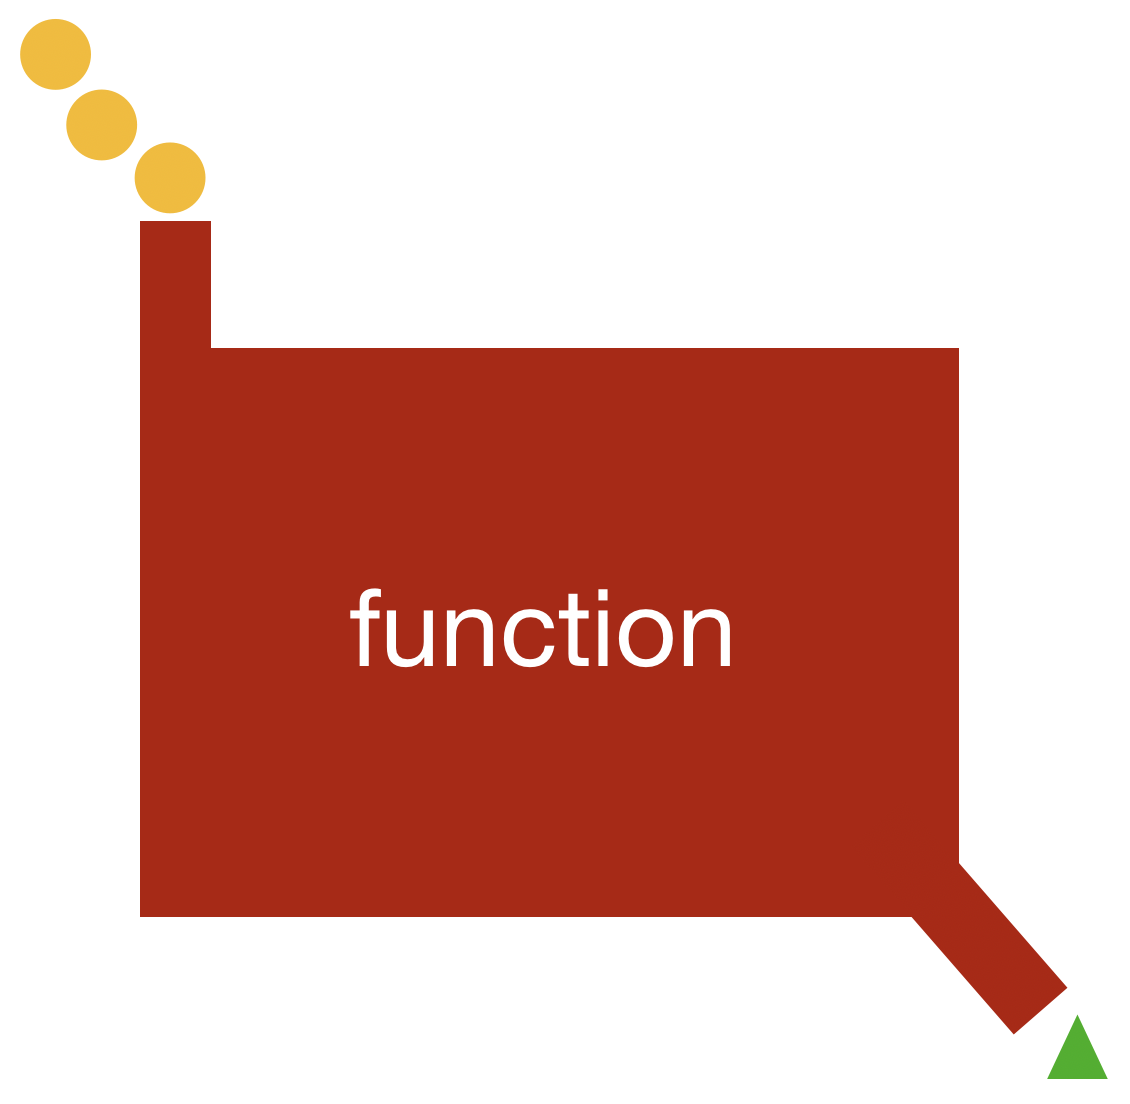
\includegraphics[width=50mm]{code-examples/function.png}
                \end{figure}
        \end{frame}

        \begin{frame}{Return}
            \begin{columns}
                \begin{column}{0.50\textwidth}
                    \inputminted[frame=single,framesep=2pt, lastline=15]{python3}{code-examples/return1.py}
                    You should call the function and assign it to a variable to hold the value.
                \end{column}
                \begin{column}{0.50\textwidth}
                    \inputminted[frame=single,framesep=2pt, lastline=15]{python3}{code-examples/return1_1.py}
                \end{column}
            \end{columns}
        \end{frame}

        \begin{frame}{Return}
            \begin{columns}
                \begin{column}{0.50\textwidth}
                    \inputminted[frame=single,framesep=2pt, lastline=15]{python3}{code-examples/return2.py}  
         %           \pause
                \end{column}
                \begin{column}{0.50\textwidth}
                    \inputminted[frame=single,framesep=2pt, lastline=15]{python3}{code-examples/return3.py}
          %          \pause
                    Return terminates the function. So, the output is 8.
                \end{column}
            \end{columns}
        \end{frame}

        \begin{frame}{Default Parameters}
            The values of parameters can be set to used as default.
            \newline
            In \textbf{\texttt{print(*args, sep=\textquotesingle \ \textquotesingle, end=\textquotesingle \textbackslash n\textquotesingle )}}, 
            sep and end are defined as default parameters.
            \inputminted[frame=single,framesep=2pt, lastline=15]{python3}{code-examples/default.py}
            \begin{columns}
                \begin{column}{0.50\textwidth}
          %          \pause
                    \inputminted[frame=single,framesep=2pt, lastline=15]{python3}{code-examples/valid1.py}  
                \end{column}
                \begin{column}{0.50\textwidth}
                    \inputminted[frame=single,framesep=2pt, lastline=15]{python3}{code-examples/valid1_1.py}                    
                \end{column}
            \end{columns}
        \end{frame}

        \begin{frame}{Default Parameters}
            The values of parameters can be set to used as default.
            \newline
            In \textbf{\texttt{print(*args, sep=\textquotesingle \ \textquotesingle, end=\textquotesingle \textbackslash n\textquotesingle )}}, 
            sep and end are defined as default parameters.
            \inputminted[frame=single,framesep=2pt, lastline=15]{python3}{code-examples/default.py}
         %   \pause
            \inputminted[frame=single,framesep=2pt, lastline=15]{python3}{code-examples/valid2.py}  
        \end{frame}

        \begin{frame}{Variadic Positional Arguments}
            It is used to let the function accept any number of arguments.
            \newline
            In \textbf{\texttt{print(*args, sep=\textquotesingle \ \textquotesingle, end=\textquotesingle \textbackslash n\textquotesingle )}}, 
            you can put as many args as you want.
            \newline 
            \newline Suppose we want a product function that works as so:
            \newline product(3, 5) gives 15.
            \newline product(3, 4, 2) gives 24.
            \newline product(3, 5, scale=10) gives 150.
            \newline 
         %   \pause
            \inputminted[frame=single,framesep=2pt, lastline=15]{python3}{code-examples/variadic.py}
        \end{frame}

        \begin{frame}{Local \& Global Variables}
            \begin{columns}
                \begin{column}{0.50\textwidth}
                    \begin{itemize}
                        \item Local variables are created in functions.
                        \item Global variables are created out of the functions.
                    \end{itemize}
                    \inputminted[frame=single,framesep=2pt, lastline=15]{python3}{code-examples/var.py}
                \end{column}
                \begin{column}{0.50\textwidth}
           %         \pause
                    \inputminted[frame=single,framesep=2pt, lastline=15]{python3}{code-examples/var2.py}                    
           %         \pause
                    \inputminted[frame=single,framesep=2pt, lastline=15]{python3}{code-examples/var3.py}                    
                \end{column}
            \end{columns}
        \end{frame}

        \begin{frame}{Local \& Global Variables}
            \begin{columns}
                \begin{column}{0.33\textwidth}
                    \inputminted[frame=single,framesep=2pt, lastline=15]{python3}{code-examples/var4.py}                    
           %         \pause
                    Prints
                    \newline 6
                    \newline 2
                \end{column}
                \begin{column}{0.33\textwidth}
          %          \pause
                    \inputminted[frame=single,framesep=2pt, lastline=15]{python3}{code-examples/var5.py}                    
           %         \pause
                    Prints
                    \newline 6
                    \newline 2
                \end{column}
                \begin{column}{0.33\textwidth}
            %        \pause
                    \inputminted[frame=single,framesep=2pt, lastline=15]{python3}{code-examples/var6.py}                    
           %         \pause
                    Prints
                    \newline 6
                    \newline 6
                \end{column}
            \end{columns}
        \end{frame}

        \begin{frame}{Lambda}
        We can write short functions in one line by using \textbf{\texttt{lambda}}.
        \newline
        \inputminted[frame=single,framesep=2pt, lastline=15]{python3}{code-examples/lambda_def.py}                    
    %    \pause
        \begin{columns}
            \begin{column}{0.50\textwidth}
                \inputminted[frame=single,framesep=2pt, lastline=15]{python3}{code-examples/lambda1.py}                    
            \end{column}
            \begin{column}{0.50\textwidth}
            %    \pause
                \inputminted[frame=single,framesep=2pt, lastline=15]{python3}{code-examples/lambda1_1.py}                    
            %    \pause
            \end{column}
        \end{columns}
        \begin{columns}
            \begin{column}{0.50\textwidth}
                \inputminted[frame=single,framesep=2pt, lastline=15]{python3}{code-examples/lambda2.py}                    
            \end{column}
            \begin{column}{0.50\textwidth}
           %     \pause
                \inputminted[frame=single,framesep=2pt, lastline=15]{python3}{code-examples/lambda2_1.py}                    
           %     \pause
            \end{column}
        \end{columns}
        \begin{columns}
            \begin{column}{0.50\textwidth}
                \inputminted[frame=single,framesep=2pt, lastline=15]{python3}{code-examples/lambda3.py}                    
            \end{column}
            \begin{column}{0.50\textwidth}
            %    \pause
                \inputminted[frame=single,framesep=2pt, lastline=15]{python3}{code-examples/lambda3_1.py}                    
            %    \pause
            \end{column}
        \end{columns}
        \end{frame}

\end{document}